\chapter{Data collection: A controlled corpus of prosodic focus marking}
\label{chapter_data}

Forming the second part of the book, the next few chapters are concerned with a study on prosodic prominence in German that is designed to explore integration in a two-fold manner: First, it concentrates on the intertwining of categorical and continuous aspects of prosodic prominence. Second, it takes into account aspects of tonal structure as well as supra-laryngeal articulation, since both have been shown to be relevant for prosodic prominence in Chapter \ref{chapter_prosody}. Special attention is going to be paid to the theoretical implications that the data reveal. Therefore, a major part of this second part of the book is going to be concerned with the development of a model that is able to explain categoriality and continuity as the outcome of a single system. This model owes a lot to the dynamical models presented in Chapter \ref{chapter_ds} and aims to contribute to a theoretical symbiosis of the categorical and the continuous aspects of speech. This symbiosis can be stated more concretely in viewing phonetics and phonology as a unified system in which ``a single formal language, nonlinear dynamics, makes it possible to model the relation between the discreteness of phonological form and the continuity of phonetic substance" \citep[937]{GafosBenus2006}. 

Building on the studies of \citet{MückeGrice2014} and \citet{Griceetal2017}, the current work investigates the expression of focus by prosodic means in a controlled laboratory setting. A large data pool was elicited that allows extensive examinations of the interplay of categorical and continuous aspects of prosodic focus marking and prosodic prominence. The following chapters describe the results obtained from the various analyses performed on the corpus and the modelling approaches designed to capture the main generalisations that the data provides for linguistic theory. Both chapters make use of the same data set, or subsets of the same data set, and employ similar measurement methods. These methods are explained in the current chapter. But before turning to the methodology, the research goals of the present study shall be stated more clearly. 

The aims pursued by the research presented in this second part of the present work can be formulated as follows: First, it will be investigated whether the relation of nuclear pitch accent type to focus type can be described as one-to-one or whether the mapping can best be characterised as fuzzy and probabilistic with different proportions of pitch accent types present in each focus type. Second, in addition to tendencies of the use of categories to differentiate focus types -- even if their distributions might not be clear-cut or non-overlapping -- the continuous aspects of the realisation of the pitch accent types will be investigated. Third, it will be examined whether there is co-variation of categorical and continuous aspects of the pitch accent patterns found in the data. Fourth, as stated above, the study will take a look beyond F0 and investigate the supra-laryngeal modifications (tongue and lip kinematics) used to express prominence and mark focus types. In this context, modifications found between unaccented and accented words as well as modifications within the group of accented words in different focus types will be considered. This last research goal is suited to contribute to our understanding of the interplay between categories and continuous modifications. Since \emph{accentuation} is conceptualised as a categorical quality of prosodic structure, it is interesting to consider whether articulatory modifications mirror this categorical nature or whether articulatory modifications are used in a continuous way to enhance prosodic prominence beyond accentuation. Furthermore, including tonal and articulatory aspects in the analysis has the potential to advance our understanding of the multiple dimensions that are recruited to express prosodic prominence.

\section{Speakers and recordings}

Twenty-seven monolingual German native speakers were recorded acoustically using a head-mounted condenser microphone and with 3D Electromagnetic Articulography (EMA) using a Carstens AG501 articulograph. The acoustic recordings were carried out with an AKG C520 headset microphone into a computer via a PreSonus AudioBox 22 VSL interface at a sampling rate of 44.1 kHz and a bit depth of 16 bit. For the EMA recordings, sensors were placed on the jaw, upper and lower lip, tongue tip, tongue blade, and tongue body to track the movements of the articulators. To compensate for head movements, reference sensors were placed on the bridge of the nose and behind the ears. A bite plate measure was used to rotate the occlusal plane. The articulatory data were recorded at 1,250 Hz, downsampled to 250 Hz and smoothed with a 3-step floating mean. In this work, the data from the lip sensors and the backmost tongue sensor are analysed.

All recordings took place at the I\emph{f}L -- Phonetik department of the University of Cologne. The speakers were aged between 19 and 35 at the time of recording. 17 of them were female, 10 were male. None of the subjects had a special training in phonetics, phonology or prosody, or reported any speech or hearing impairments. The participants received compensation for their participation in the study. The recording session, after the participant had been prepared, lasted about 45 minutes including a training session.

The participants were involved in an interactive animated game sitting in front of a computer screen. They were told that the game revolved around two robots working in a factory. One of the robots likes to move around the tools while the other, slightly older and technologically outdated, needs the participant's help to retrieve these tools. In each trial, the participant first saw one robot placing the tool on an object in the factory room and leaving the scene. In the next step, the second, older robot entered the scene. This robot did not enter the factory room but stopped in front of the closed door asking a question about the action of the first robot. After the participant's answer, the door opened and the second robot entered the room, took the tool, and left the scene.

\section{Speech material}

Natural productions by a male, native German speaker were used for the robot's questions that served as triggers for the focus structures of the answers. They were chosen such that the target word denoting the object (where the tool is placed) could be in broad focus, narrow focus, contrastive focus, or in background (with a contrastive focus on the direct object). 

Table \ref{tab:focus_trigger_target} shows examples for such question-answer-pairs. In the examples, square brackets and subscript $F$ mark the focus domain. Each question was given auditorily and additionally shown as a combination of pictures in a thought bubble above the robot's head: the question tool on top of the question object in the case of background and contrastive focus; a simple question mark in the case of broad focus; the object and the question word ``wo?" (`where?') in the case of narrow focus. The answers that the participant had to produce were presented in written form at the bottom of the screen. Many participants reported that they were able to give the answers without reading them on the screen after some trials. The participants were asked to always produce the answer with the same syntactic structure and to not add any words like ``nein" (`no'). None of the participants had any problems with this restriction. Likewise, none of the participants reported that they found the sentences unnatural or difficult.

\begin{table}
\caption{Example question-answer-pairs to elicit the focus structures.}
\label{tab:focus_trigger_target}
\begin{tabularx}{\textwidth}{l Q}
	\lsptoprule
Focus structure & Example trigger (Q) and target sentence (A) \\
\midrule
Background & Q: Hat er die Säge auf die Wohse gelegt? \\
& \hspace{5 mm}`Did he put the saw on the Wohse?' \\
& A: Er hat [den Hammer]$_F$ auf die Wohse gelegt. \\
& \hspace{5 mm}`He put the hammer on the Wohse.'\\
& \\
Broad focus & Q: Was hat er gemacht? \\
& \hspace{5 mm}`What did he do?' \\
& A: Er hat [den Hammer auf die Wohse gelegt.]$_F$ \\
& \hspace{5 mm}`He put the hammer on the Wohse.' \\
& \\
Narrow focus & Q: Wo hat er den Hammer hingelegt? \\
& \hspace{5 mm}`Where did he put the hammer?' \\
& A: Er hat den Hammer [auf die Wohse]$_F$ gelegt. \\
& \hspace{5 mm}`He put the hammer on the Wohse.' \\
& \\
Contrastive focus & Q: Hat er den Hammer auf die Mahse gelegt? \\
& \hspace{5 mm}`Did he put the hammer on the Mahse?' \\
& A: Er hat den Hammer auf [die Wohse]$_F$ gelegt. \\
& \hspace{5 mm}`He put the hammer on the Wohse.'\\
\lspbottomrule
\end{tabularx}
\end{table}

To control for the segmental context and for word frequency, twenty German sounding disyllabic nonce words with a C$_1$V$_1$:C$_2$ǝ structure were chosen as target words. The words were designed to have word stress on the first syllable. The stressed vowel V$_1$ was either /a:/ or /o:/, the second vowel always schwa. The consonants (C$_1$ and C$_2$) either require movements of the labial system or the tongue tip to avoid influences on the tongue body measures for the vowel. The first consonant was chosen from the set of /n m b l v/, the second consonant from /n m z l v/. The consonants and vowels were combined such that each first consonant C$_1$ of /n m b l v/ occurred twice with each first vowel V$_1$ /a:/ or /o:/. Each second consonant-schwa-combination /nǝ mǝ zǝ lǝ vǝ/ occurred four times in the whole set. Special care was taken that the words did not overlap with real German words. All words were presented with the female determiner ``die" /di:/. All participants pronounced the words as expected. The target words are listed in Table \ref{tab:target_words}.

\begin{table}
\caption{Target words.}
\begin{tabularx}{\textwidth}{XXXXl}
\lsptoprule
Nohme & Mohme & Bohme & Lohne & Wohme \\ 
Nohse & Mohwe & Bohwe & Lohle & Wohse \\ 
Nahne & Mahne & Bahle & Lahse & Wahne \\ 
Nahle & Mahse & Bahwe & Lahle & Wahwe\\
\lspbottomrule
\end{tabularx}
\label{tab:target_words}
\end{table}

In the setting of the experiment, each target word was associated with a fictitious visual object. The association remained fixed throughout the whole experiment and across all participants. There was no connection between the appearance of the object and the sound of the word. The participants were presented with all objects and target words in a preparation phase immediately before the experiment and were asked to read the words aloud with the determiner ``die" (``die Nohme", ``die Lahse", etc.). This phase lasted a few minutes and was included to ensure that no participant placed the stress on the second syllable or had any difficulties pronouncing the words. All participants placed word stress on the first syllable starting with the first production.

\begin{table}[t]
	\caption{Tools with English translation.}
	\begin{tabularx}{\textwidth}{XlXl}
		\lsptoprule
		Tool & Translation & Tool & Translation \\
		\midrule
		Amboss & anvil & Pinsel & Paint brush \\
		Besen & broom & Rolle & Paint roller \\ 
		Bohrer & drill & Säge & Saw \\
		Bürste & brush & Schere & Scissors \\
		Hammer & Hammer & Zange & Pliers\\
		\lspbottomrule
	\end{tabularx}
	\label{tab:tools}
\end{table}

As described above, in each trial, a tool is placed on one of the fictitious objects. Each object was paired with a tool to occur with. All tools are given in Table \ref{tab:tools}. Since there were 10 tools and 20 target words in the game, each tool had to occur twice. Furthermore, for the background condition and the contrastive focus condition, a competitor tool or object was needed: for the direct object of the question when the target word was in the background (``Did he place X on A?” “He placed Y on A!”) and for the indirect object of the question when the target word was in contrastive focus (``Did he place X on A?” “He placed X on B!"). These combinations were fixed for all participants, yielding 20 quadruples of target object, tool, competitor object, and competitor tool.\footnote{In the case of trials with broad focus or narrow focus, the competitor object and the competitor tool are not needed. Thus, in the quadruples for broad and narrow focus trials, these positions are empty.} The competitor object was chosen randomly with the restriction that the first consonant or the first vowel did not equal the first vowel or consonant of the target object. The competitor tool was selected such that it differed in the first consonant from the target sentence tool. The 20 target words occurred with all four focus conditions resulting in 80 trials per speaker. As a training phase, 16 trials with different objects and tools (everyday objects, e.g. a table) preceded the actual experiment session. 



For each of the 27 participants the order of trials was randomised with some restrictions: Subsequent trials were not allowed to contain the same target word or tool used in the target sentence. Furthermore, there were no three subsequent trials with the same focus condition. For two subsequent trials with identical focus condition an upper limit was set: In only 15\% of the list, two adjacent trials with equal focus conditions occurred.

The scenes, objects, tools, and robots were drawn by a professional book illustrator. The game was developed as an interactive website using HTML and JavaScript with jQuery for animation (e.g. robots' arm and mouth movement, the door opening, and closing). The experimenter sat behind the participant and pressed a key on the keyboard to make the robot move toward the tool and proceed to the next trial. There was a ``rescue key" to repeat the trial in case something went wrong. Between trials, the scenery disappeared for 4 seconds and the screen transitioned through a series of light, muted colours. This short break detached the trials from one another to make sure that the focus structure of the target sentence made reference to the current trial only and not to the previous trial. In order to make the task more game-like, points were counted for each complete trial in the lower right corner of the screen. Figure \ref{fig:exp_trial} presents an example of the experiment screen where the second robot has just asked his question and is waiting for the answer of the participant. The code of the experiment app is available under open source and creative commons license: \href{http://doi.org/10.5281/zenodo.2611287}{http://doi.org/10.5281/zenodo.2611287}.

\begin{figure}
\fbox{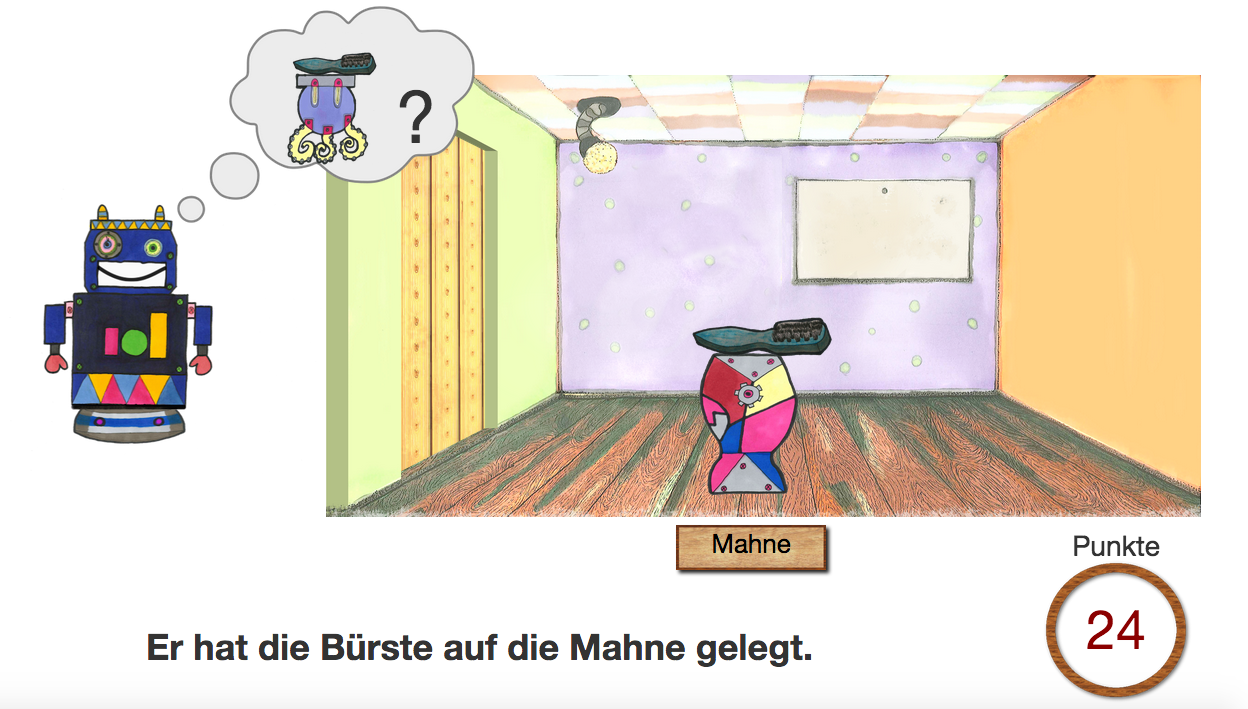
\includegraphics[width=.95\textwidth]{figures/ch5/Exp_Trial.png}}
\caption{Example screen from the experiment during a trial with contrastive focus condition.}
\label{fig:exp_trial}
\end{figure}

\section{Measures}

This section describes the various measures performed on the data set. All measures are in some form based on the annotation of the stressed syllable and the vowel of the stressed syllable. One trained annotator labelled the beginning and end of the stressed syllable of each target word using the waveform and the spectrogram in the emuR speech database system \citep{Winkelmannetal2018}. Another trained annotator labelled the beginning of the vowel of this syllable in Praat \citep{BoersmaWeenink2018}. 

\subsection{Tonal onglide}

To assess the differences in the F0 contours, the tonal onglide of each nuclear pitch accent was measured. Figure \ref{fig:onglide_measure} provides a schematic depiction of the tonal onglide measure. The tonal onglide characterises the portion of the F0 movement towards the main tonal target of the pitch accent \citep{RitterGrice2015}. In terms of an autosegmental-metrical analysis, like GToBI \citep{GriceBaumannBenzmüller2005}, L+H* and H* pitch accent types are described by a rising movement and result in positive onglide values. In contrast, the accent types H+L* or H+!H* are described by a falling movement from the initial high portion of the accent down to the L* or !H* on the accented syllable and result in negative onglide values. In addition to capturing the direction of the tonal movement (``is it rising or falling?"), the tonal onglide reflects the magnitude of the rise or fall in semitones (``how much does it rise or fall?"). Albeit being a continuous variable that represents both the direction of the pitch movement as well as the magnitude of this movement, the tonal onglide does not capture all relevant details of pitch accents \citep{Griceetal2017}. Nevertheless, it has been shown that the tonal onglide movement is a perceptually relevant parameter of pitch accents in German \citep{BaumannRöhr2015, RitterGrice2015}.

F0 movements were annotated by two labellers with training in prosody using a simple labelling scheme without having access to the intended focus structures of the sentences. First, the labellers identified all utterances in which the speaker did not place the nuclear pitch accent on the object. Only cases which exhibited a clear nuclear accent on the target word for both annotators were labelled as accented. Second, the labellers judged perceptually whether the nuclear pitch accent was falling or rising. Third, the labellers identified the beginning and the end of the onglide movement manually within a window of three syllables including the accented syllable in the centre, the syllable before and the syllable after the accented syllable.

For rising accents, a local minimum just before the rising movement was annotated in the pre-accented syllable or the accented syllable itself as the beginning of the onglide movement. A local maximum at the end of the rise was labelled in the accented syllable or the post-accented syllable as the end of the movement. For falling accents, a relatively high point at the start of the fall was labelled in the pre-accented syllable or the accented syllable itself as the beginning of the onglide movement. Since F0 is usually falling throughout the syllable in a falling accent and hence a tonal target is virtually impossible to determine, the midpoint of the vowel of the accented syllable was marked as the end of the accentual movement.

If the nuclear accent was not placed on the target word, it was placed on the direct object of the sentence. In this case, the part of the phrase containing the target word and the following verb is characterised by a low stretch of F0. This situation -- deaccentuation of the target word -- was found in almost all cases of the background condition and in a minority of cases of the other conditions. When deaccentuation of the target word occurred, an ``onglide” measure was carried out with fixed time points (5 ms before the start and 50 ms before the end of the stressed syllable). It is not possible to speak of tonal onglide in a strict sense here since there is no tonal movement of a pitch accent. Hence, there is no beginning and end of a tonal movement that can be identified. However, this measure makes it possible to compare and model the intonation of all utterances, with accented and unaccented target words, and to relate the intonational and articulatory modifications used to express focus structure across all experimental conditions.

Although using the semitones scale already eliminates a great deal of variation between speakers, like gender effects, normalisation is needed to make the speakers more comparable. To do so, each rising onglide value is divided by the mean of the speaker’s rising onglides, and each falling onglide value is divided by the mean of the speaker’s falling onglides. It is plausible that a rise is best interpreted in relation to other rises, while a fall is best interpreted in relation to other falls of the same speaker. For example, a raw onglide value of +6 semitones might be quite extreme for a speaker with a mean of +4 semitones for rises compared to a speaker with a mean of +6 semitones for rises. For the unaccented cases, where it is not possible to speak of rises and falls, the overall mean of the absolute onglide values for each speaker was used in the normalisation procedure.

\begin{figure}
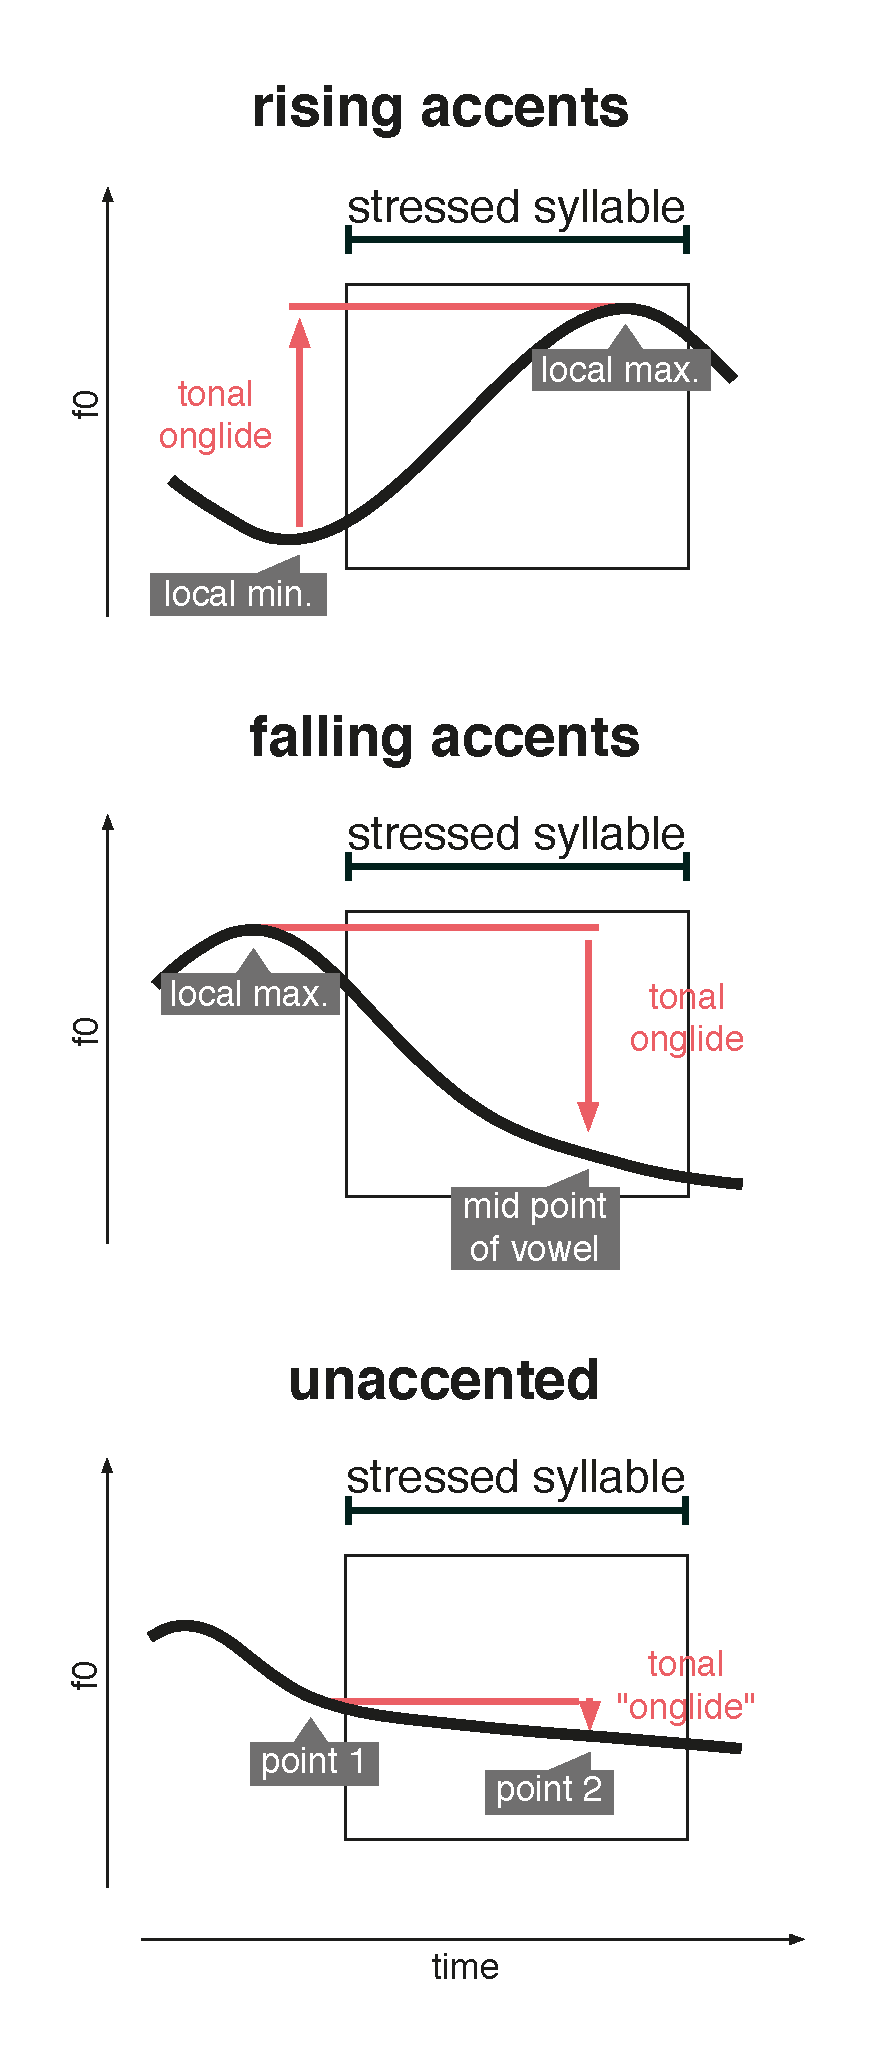
\includegraphics[width=7cm]{figures/ch5/measures_onglide.pdf}
\caption{Schema of tonal onglide measure.}
\label{fig:onglide_measure}
\end{figure}

\subsection{Alignment of the peak}

The labels described above for the tonal onglide were used to determine the alignment of the peak. In the case of falling accents, the beginning of the fall was used as the peak; in the case of rising accents, the end of the rise was used as the peak. The alignment of the peak is calculated as the difference between the time point of the peak and the time point of the beginning of the vowel in the accented syllable in ms. No equivalent for deaccented target words could be applied for this measure. Figure \ref{fig:alignment_measure} shows a schema of the measure.

\begin{figure}
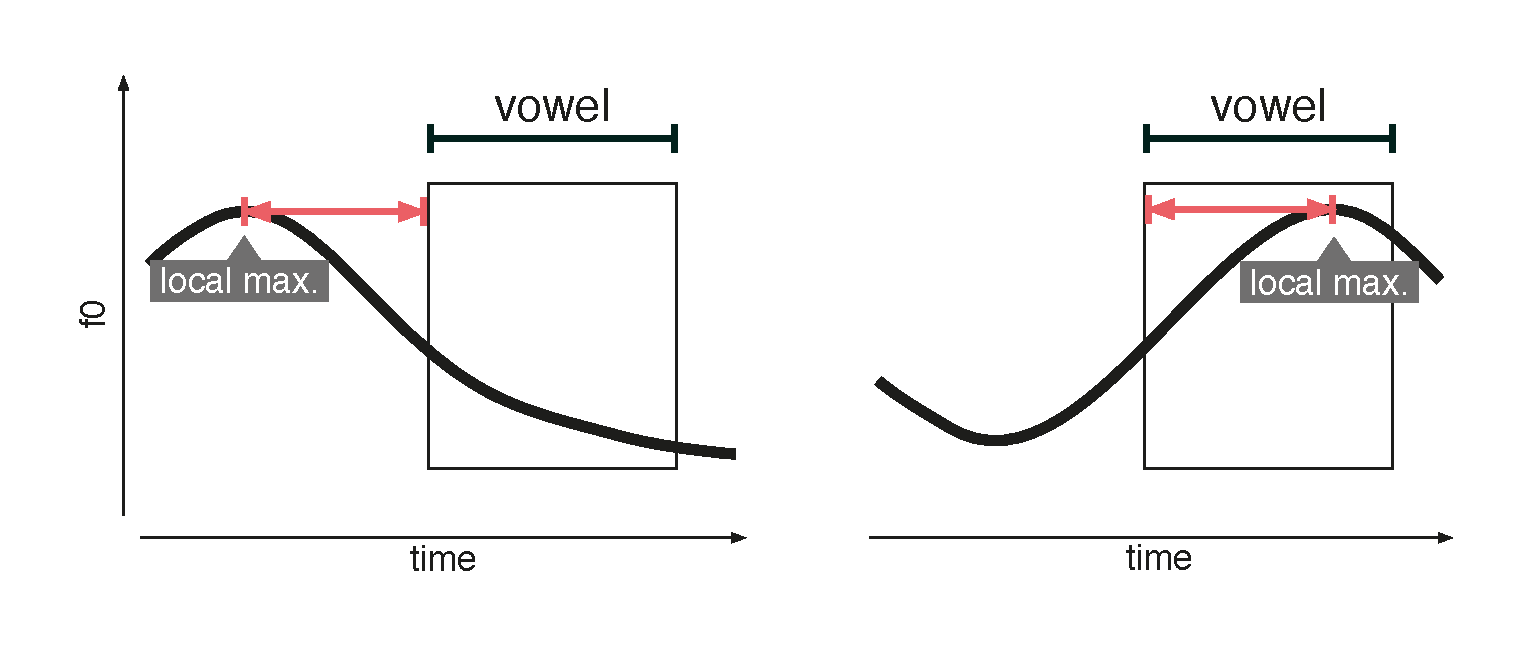
\includegraphics[width=\textwidth]{figures/ch5/measures_alignment.pdf}
\caption{Schema of alignment measure.}
\label{fig:alignment_measure}
\end{figure}

\subsection{Lip aperture}

Lip aperture was evaluated as the Euclidean distance between the lips, as given in Equation \ref{eq:eukl_lips} \citep{Byrd2000}, within the boundaries of the syllable. An automatic procedure was used to determine the maximum of the trajectory within the boundaries of the labelled acoustic syllable. The maximal lip aperture represents the widest opening of the lips during the production of the vowel. Figure \ref{fig:lip_measure} presents a schema of this measure.

\begin{equation}
\begin{split}
\text{lip aperture } x &= \text{upper lip } x - \text{lower lip } x\\
\text{lip aperture } y &= \text{upper lip } y - \text{lower lip } y\\
\text{lip aperture} &= \sqrt{(\text{lip aperture } x)^2+(\text{lip aperture } y)^2}
\end{split}
\label{eq:eukl_lips}
\end{equation}

\begin{figure}
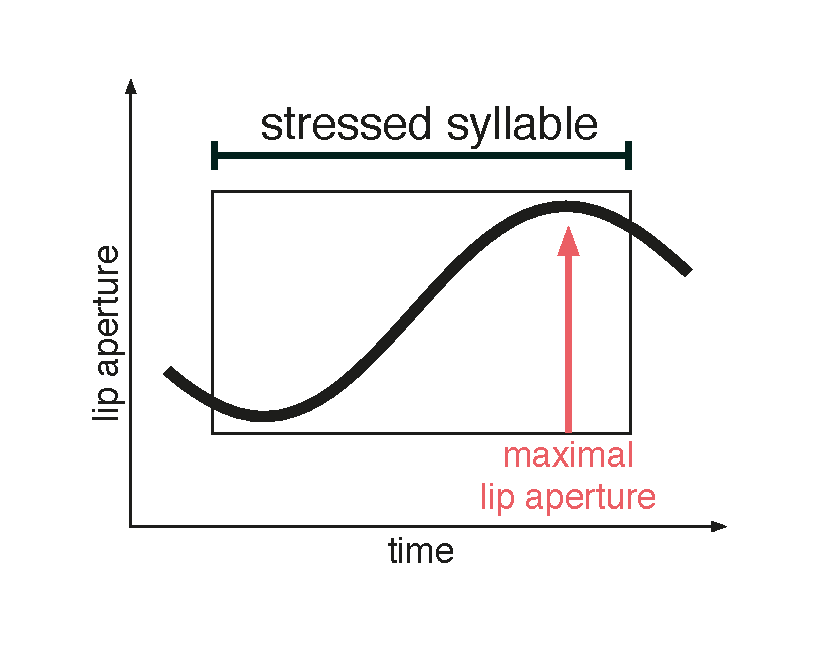
\includegraphics[width=7cm]{figures/ch5/measures_lips.pdf}
\caption{Schema of the lip aperture measure.}
\label{fig:lip_measure}
\end{figure}

\subsection{Position of the tongue body}

The vertical (high-low) and the horizontal (front-back) position of the back-most tongue sensor was measured as an indication of the position of the tongue body. Because the stressed syllable is followed by a syllable containing schwa, the exact target of the horizontal tongue body movement could not consistently be determined for the vowel /o/ in the stressed syllable as schwa can be lower than /o/. Therefore, a different method was applied for all tongue trajectory measures: The first 50\% of each acoustic vowel was taken as a time window to measure the tongue body position. The mean of all points on the trajectory falling in this 50\% window was calculated for each token. The length of the window (50\%) is, of course, arbitrary. However, it seems plausible to assume that the acoustic vowel is a perceptually relevant time interval. It thus makes sense to ask how high or low, back or front the vowel is articulated in this window. Using only the first 50\% reduces the influence of the following vowel on the measure. Figure \ref{fig:tounge_measure} shows a schema of the measure for two different trajectories and the potential outcome of the measure (as bar graphs). The measure was used on both the horizontal and the vertical dimension of the movement as well as for both vowels /a/ and /o/ to make all measures comparable.

\begin{figure}
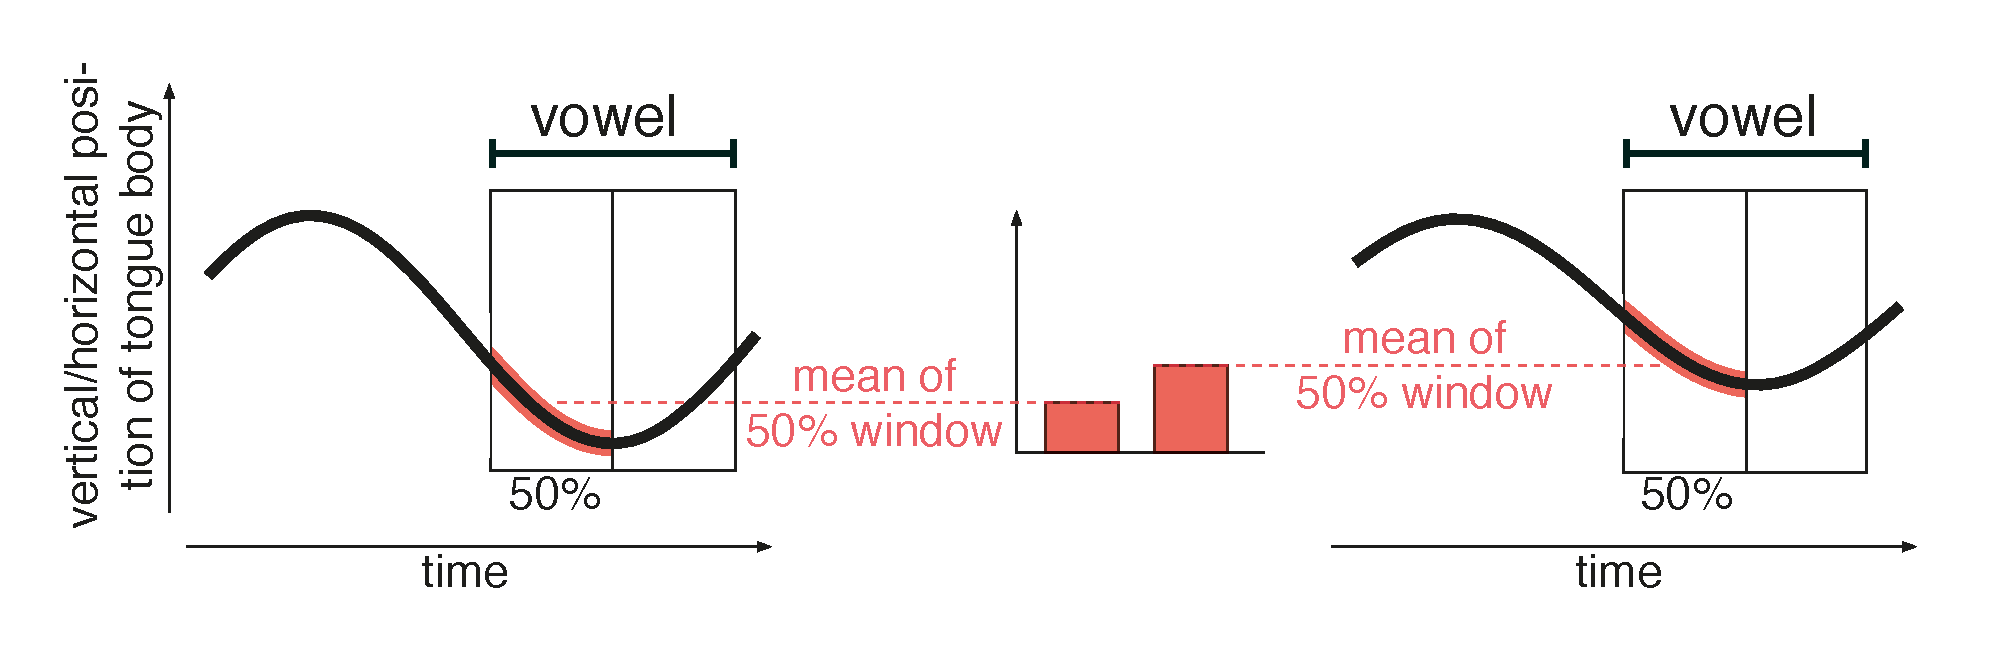
\includegraphics[width=\textwidth]{figures/ch5/measures_tbo2.pdf}
\caption{Schema of the tongue body measure.}
\label{fig:tounge_measure}
\end{figure}

\section{Data and availability}

Of the 2160 planned utterances (80 utterances per speaker, 27 speakers), 29 (1.3\%) productions had to be excluded due to technical problems during the recording or because the participant did not pronounce the words of the sentence correctly (and the trial was not repeated). The total dataset comprised 2131 recordings. 

As stated above, the target word is unaccented in the background condition in the majority of cases. Conversely, the target word is accented in the majority of cases in all other conditions (broad focus, narrow focus, and contrastive focus). This situation was expected and planned in the design of the study (see Chapter \ref{chapter_prosody}). The opposition background vs. \{broad focus, narrow focus, contrastive focus\} is used for the comparison of unaccented and accented. Therefore, all tokens with accented target words are excluded from the background condition (0.14\% of the productions in the complete corpus of 2131 utterances). Likewise, all tokens with unaccented target words are excluded from the conditions broad focus, narrow focus and contrastive focus (1.88\% of the productions in the complete corpus of 2131 utterances). It has to be noted that only those cases were labelled as accented that exhibited a clear nuclear pitch accent on the target word for both annotators. All in all, 2088 utterances enter the analysis, i.e. 96.67\% of the 2160 planned utterances. The data set is accessible for download: \href{https://osf.io/4g6s2/}{https://osf.io/4g6s2/}.

